\documentclass{article}
\usepackage[]{graphicx} % Required for inserting images
\usepackage{amsfonts}
\usepackage[margin=2.5cm]{geometry}
\usepackage{mathptmx}
\usepackage{amsthm}
\usepackage[utf8]{inputenc}
\usepackage[T1]{fontenc}
\usepackage{listings}
\usepackage{mathtools}
\usepackage{pdfpages}
\usepackage{bbold}
\usepackage{hyperref}
\usepackage{fancyhdr}
\usepackage{minted}
\usepackage{color}
\usepackage{url}
\usepackage{hyperref}
\usepackage{subcaption}
\usepackage[colorinlistoftodos]{todonotes}
\usepackage[backend=biber,style=alphabetic,]{biblatex}
\usepackage[T1]{fontenc}
\usepackage{lmodern}
\pagenumbering{arabic}
\usepackage{amsthm}
\usepackage{todonotes} % define the \todo block useful for comments
\author{TENA Arthur}
\date{ }
\usepackage[tikz]{bclogo}
\usepackage{xcolor}

\begin{document}
\begin{titlepage}

\newcommand{\HRule}{\rule{\linewidth}{0.5mm}}
\center 


\begin{figure}
    \centering
    \includegraphics[width=0.7\linewidth]{SSD.png}
\end{figure}



\textsc{\Large Master 2 Statistiques et Sciences des Données }\\[1cm] % Major heading such as course name
\HRule \\[0.4cm]
{ \huge \bfseries TP3 SVM ML }\\[0.4cm]
\HRule \\[1.5cm]
\begin{center}
\begin{Large}

TENA Arthur\\
\hspace{4cm}

\end{Large}
\end{center}
    


\begin{figure}[b]
    \centering
    \includegraphics[width=0.25\linewidth]{UM.png}
    \label{UM}
\end{figure}
\begin{Large} Année 2024 - 2025 \\
\end{Large}

\end{titlepage}
\pagebreak
\renewcommand{\contentsname}{Sommaire}
\tableofcontents
\thispagestyle{empty}
\newpage

\maketitle

\section{Introduction}
Le \underline{Support Vector Machine} (SVM) est une méthode d'apprentissage supervisé principalement utilisée pour les tâches de classification et, dans certains cas, de régression. 

L'idée principale du SVM est de trouver une frontière ou un hyperplan qui sépare au mieux les différentes classes de données dans un espace à plusieurs dimensions. Pour un problème de classification binaire (deux classes), le SVM cherche à maximiser la marge entre les points les plus proches des deux classes et l'hyperplan séparateur (voir figure \ref{fig1}).

Les vecteurs de support sont les points de données qui se trouvent le plus près de l'hyperplan. Ces points déterminent la position et l’orientation de l'hyperplan, car ce sont eux qui contraignent la marge. La marge est définie comme la distance entre ces points critiques et l'hyperplan.


Nous allons dans un premier temps regarder quelques applications simple de la méthode SVM avec le data set \textit{iris}, puis nous verrons un exemple de classification de visages 

\begin{figure}[H]
    \centering
    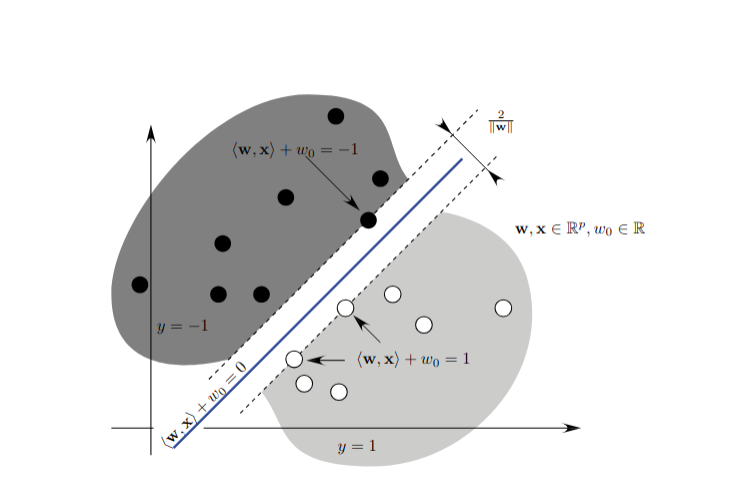
\includegraphics[width=0.5\linewidth]{SVM.png}
    \caption{ Marge et hyperplan séparateur dans le cadre de classes séparables (cas d’un noyau linéaire)}
    \label{fig1}
\end{figure}

\section{Exemples d'applications}
\subsection{Question 1}

Le score sur les données d'entraînements est de 0.74 ce qui signifie que le modèle à classifié correctement 74\% des exemples de l'ensemble de test ou de validation.\\
Le score obtenu sur les données de test est de 0,66, ce qui correspond à un taux de classification correcte de 66 \%. Cela indique que le modèle a moins bien réussi à classer les données de test par rapport aux données d'entraînement ou de validation.\\
Nous pouvons donc nous dire que la classification linéaire est "trop simple" est qu'un autre noyau est peut être plus adapté à nos données. C'est ce que nous allons voir dans la question 2 avec un noyau polynomial.
\subsection{Question 2}
Nous nous retrouvons maintenant avec un score de 0.7 avec un noyau polynomial pour les données d'entraînement et un score de 0.76 pour les données de tests. C'est mieux que pour le noyau linéaire pour les données de tests mais moins bon pour les données d'entraînement.
\subsection{Visualisation de la classification}

\begin{figure}[H]
    \centering
    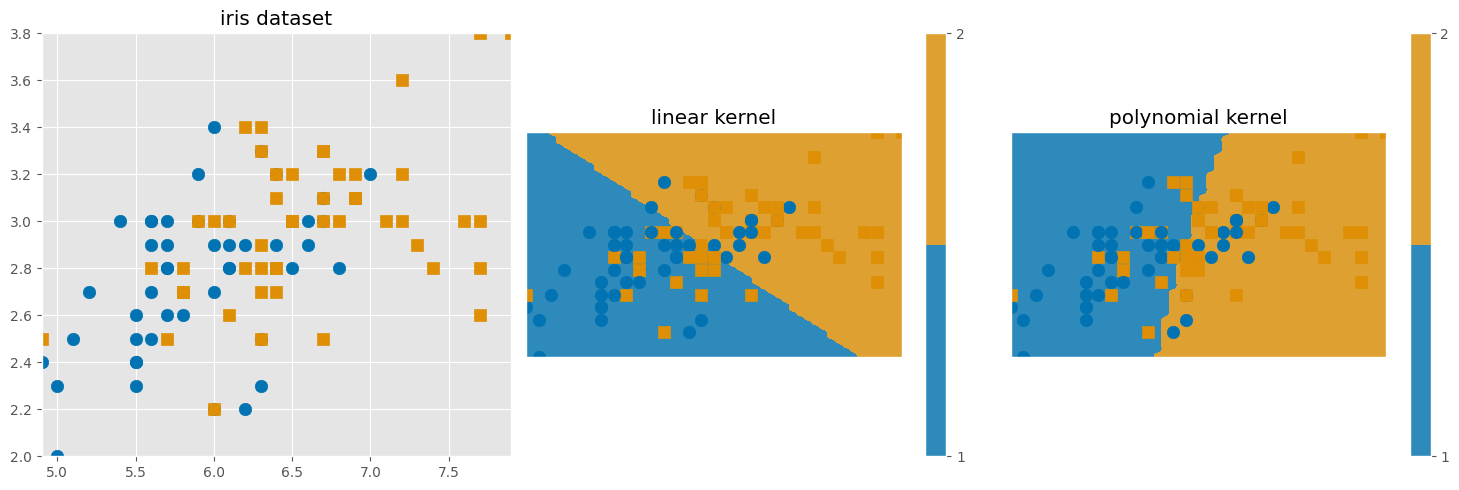
\includegraphics[width=0.75\linewidth]{Visualisation_q2.png}
    \caption{Visualisation du jeu de donnée et des 2 premières questions}
    \label{fig2}
\end{figure}

- Le graphique de gauche représente notre jeu de donnée 'Iris' et plus particulièrement, la variable "sepal.width" de Iris.\\
- Le graphique du milieu corresponds à la classification du jeu de donnée par la méthode SVM avec un noyau linéaire. La ligne diagonale représente la frontière de séparation linéaire entre les deux classes. Les zones colorées en bleu et orange correspondent aux régions où le modèle prévoit chaque classe.On remarque que la frontière est une ligne droite, ce qui est caractéristique d'un noyau linéaire. Cependant, on observe également que plusieurs points de chaque classe se trouvent de l'autre côté de la frontière, ce qui indique que le noyau linéaire a du mal à séparer parfaitement les classes qui se chevauchent.\\
- Le graphique de droite corresponds à la classification du jeu de donnée par la méthode SVM avec un noyau polynomial. On peut voir que la région en bleu et orange est moins simplement séparée, et le modèle semble mieux classer certains des points proches de la frontière par rapport au modèle linéaire.\\

\textbf{Conclusion :} Le noyau polynomial nous semble plus adapté aux différents jeu de données car il est plus complexe et permet une plus grande flexibilité pour la frontière car n'étant pas forcément linéaire. Cependant, dans notre cas, nous avons observé que la différence entre les deux scores n'était pas significative. Cela pourrait s'expliquer par la variable "sepal.width" du jeu de données Iris, qui permet une bonne séparation des deux classes à l'aide d'une simple ligne droite.

\newpage

\section{Classification des visages }
L'exemple suivant est un problème de classification de visages. Nous utilisons une base de donnée qui nous a été fournie et dans cette partie, nous nous concentrerons sur 2 personnes : 'Tony Blair' et 'Colin Powell'.

\subsection{Question 4}
Nous avons ici 12 visages correspondant à ces 2 personnes.

\begin{figure}[H]
    \centering
    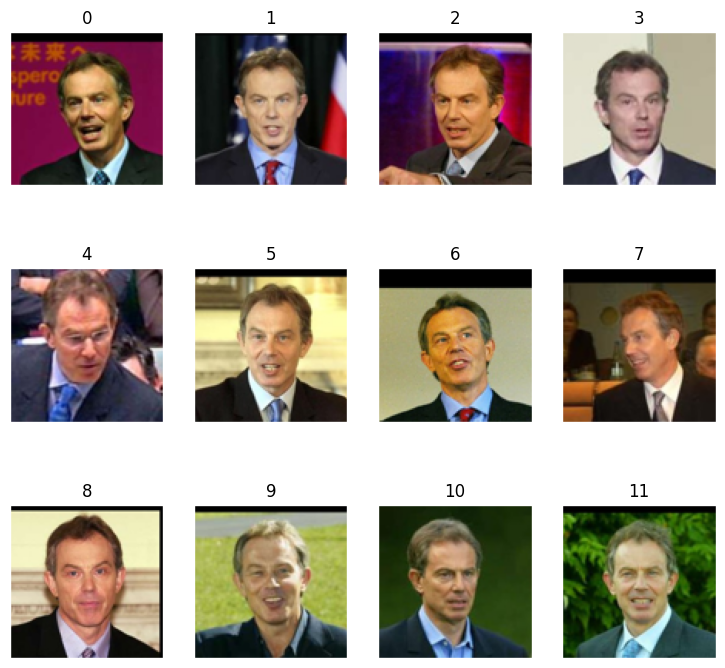
\includegraphics[width=0.75\linewidth]{Visages.png}
    \caption{Visages utilisé dans notre étude}
    \label{fig3}
\end{figure}

\underline{\textit{Rappels} :} \\
- Le score est le pourcentage de classification correcte. L'erreur est donc calculée en faisant 1-score.\\
- Le paramètre C contrôle la complexité du classifieur dans la mesure où il détermine le coût d’une mauvaise classification : plus C est grand, plus la règle obtenue est complexe (le nombre de points pour lesquels on veut minimiser l’erreur de classification croît).\\

Nous allons maintenant montrez l’influence de ce paramètre de régularisation C en le faisant varier sur une échelle logarithmique entre 1e5 et 1e-5.\\

\begin{figure}[H]
    \centering
    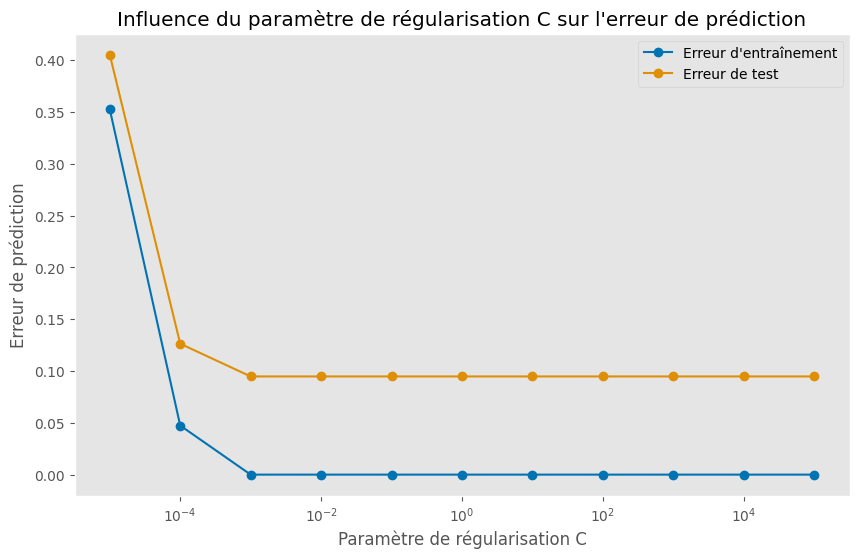
\includegraphics[width=0.75\linewidth]{erreur_C.png}
    \caption{Influence du paramètre C sur l'erreur de prédiction}
    \label{fig4}
\end{figure}

Quand la valeur de C est petite l'erreur sur les données d'entrainement et de test est grande (dee l'ordre de 0.4) et plus la valeur de C augmente, plus l'erreur diminue pour se stabilisé à 0.1 pour l'erreur sur les données de test à partir de C= 1e-3. Cette tendance est aussi vérifié pour l'erreur sur les données de tests, mais cette fois, l'erreur se stabilise autour de 0 à partir de C=1e-3.\\
C'est ce que nous avons vu plus haut avec le score sans variable de nuissance où nous avions un score qui se stabilisait à 1 et un score sur les données d'entrainement d'environ 0.93.

\newpage
\subsection{Question 5}
Nous allons voir maintenant l'influence des variables de nuissance sur le score. \\

\begin{figure}[H]
    \centering
    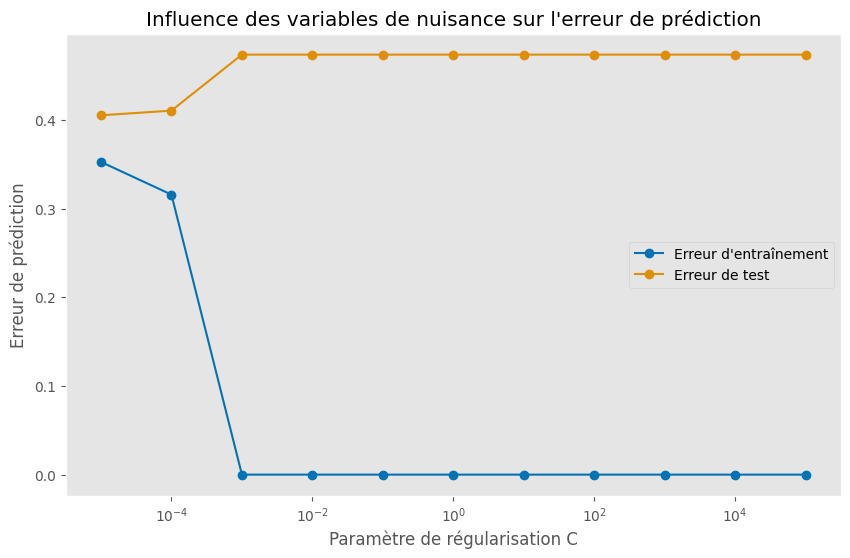
\includegraphics[width=0.75\linewidth]{erreur_c_nuissance.png}
    \caption{Influence du paramètre C sur l'erreur de prédiction sur un jeu de donnée content des variables de nuissance}
    \label{fig5}
\end{figure}

On remarque tout d'abord que le score a drastiquement diminué, il atteint 0.61 pour le score de test et 0.64 pour le score sur les données d'entraînement.\\
Sur le graphique, nous nous rendons compte de l'influence du paramètre de régularisation, une nouvelle fois, l'erreur de précision sur les données d'entraînement se stabilise à 0 à partir de C=1e-3. Pour l'erreur sur les données de test par contre, il se stabiliuse autour de 0.45 à partir de C=1e-2. Cela suggère que le modèle est trop influencé par les variables de nuisance.

\subsection{Question 6}
Nous allons maintenant essayer d'améliorer la prédiction à l'aide d'une réduction de dimension basé sur la PCA.\\

Sur mon ordinateur, je voulais regarder l'influence du nombre de composants sur l'erreur de prédiction des données d'entraînement et de tests en prennant $n_{comp}=\{5,10,20,50\}$ mais c'était trop long à compiler (980min), je vais donc utiliser les valeurs d'un camarade pour ma question.\\


\begin{table}[H]
    \centering
    \begin{tabular}{|c|c|c|}
    \hline
       $n_{comp}$  & score test & score entraînement \\
    \hline
       5  & 0.605 & 0.616  \\
    \hline     
      10   & 0.605  &  0.637 \\
    \hline     
       15  & 0.653 & 0.589  \\
    \hline     
      20   & 0.658 &   0.589 \\
    \hline
       25  & 0.695 &  0.584 \\
    \hline
       80  & 0.747 & 0.489  \\
    \hline
      120  & 1.0 &  0.526 \\
    \hline
      200  & 0.926 &  0.521 \\
    \hline
    \end{tabular}
    \caption{Table récapitulative du score selon le nombre de composantes principales}
    \label{tab1}
\end{table}

On observe que, globalement, l'augmentation du nombre de composantes principales ($n_{comp}$) améliore le score sur les données de test jusqu'à un certain point.\\
Le score sur les données d'entraînement varie peu au début, mais se dégrade fortement pour les valeurs plus élevées.\\

À partir de 15 composantes, les scores de test commencent à s'améliorer nettement, atteignant un maximum autour de 120 composantes avec un score de test de 1. Ceci étant, pour un score de 1 sur les données tests, nous avons seulement 0.526 sur les données d'entraînement. Ce qui pourrait être expliqué par un surrajustement sur les données de tests.\\

Au final, un bon compromis serait de prendre environ 80 composantes principales et de continuer des tests avec un nombre de composantes variant autour des 80. 


\section{Conclusion}
Nous avons regarder l'influence de plusieurs paramètres de la méthode SVM comme le noyau, le paramètre de régularisation ou la réduction de dimension. Le choix du noyau nous semble important bien que nous n'en ayant vu que 2 (linéaire et polynômiale) et dépends du jeu de données à étudié, dans notre cas le noyau linéaire était suffisant bien que le noyau polynômiale améliorait un peu la prédiction.\\

Pour ce qui est de l'influence du paramètre de régularisation C, nous avons vu une drastique augmentation du score (ou diminution de l'erreur) qui se stabilise à partir de 1e-3, pour les données d'entraînement que ce soit avec ou sans variable de nuissance. Sur les données de test, les variables de nuissance affectent beaucoup le score qui ne semble. Une ACP nous semblait alors une bonne chose à faire.\\

Nous avons ensuite vu l'influence du choix de composantes principales à garder dans une ACP afin d'y évaluer la précision de la prédiction. Un choix qui va beaucoup dépendre du jeu de données. 


\end{document}
